% Correcting the title chapter page
\fancypagestyle{plain}{%
    \fancyhf{}
    \fancyhead[RO,LE]{\bfseries \thepage}
    \fancyhead[CO]{\rightmark}
    \fancyhead[CE]{\leftmark}
    \renewcommand{\headrulewidth}{0.4pt}}

\chapter{Grupe - opći pojmovi}

\section{Definicija grupe i primjeri}


Moć teorije grupa leži u njenoj apstraktnosti koju je poznati fizičar Arthur
Eddington ilustrirao 
riječima
\begin{quote}
\emph{Potrebna nam je super-matematika u kojoj su operacije jednako nepoznate kao i
veličine na koje te operacije djeluju, te super-matematičar koji ne zna što radi kada
izvodi te operacije. Takva super-matematika je teorija grupa.}
\end{quote}
Možda je Eddingtonova karakterizacija teorije grupa kao "super-matematike" malo pretjerana, jer
teorija grupa je čvrsti dio standardne matematike, ali točno je da je upotrebljivost
ove teorije iznenađujuće široka i da najraznolikiji matematički i fizikalni objekti
imaju strukturu grupe.
Stoga je poželjno prvo definirati pojam grupe maksimalno apstraktno, bez pozivanja
na njene konkretne primjere i realizacije:

\begin{definicija}[Grupa] 
Grupa $(G,\star)$ je skup objekata $G$ na kojem je definirana binarna operacija
 $\star$ tako da su zadovoljena sljedeća svojstva:
\begin{enumerate}
\item $g_1 \star g_2 \in G \quad \forall  g_1, g_2 \in G$  (zatvorenost)
\item $ g_1 \star (g_2 \star g_3) = (g_1 \star  g_2)\star g_3 \quad \forall 
    g_1, g_2, g_3 \in G$  (asocijativnost)
\item $\exists e \in G \td g\star e = e \star g = g \quad \forall g\in G$
    (egzistencija jedinstvenog identiteta)
\item $\forall g\in G \;\; \exists g^{-1} \td g\star g^{-1} = g^{-1}\star g =e$
    (egzistencija inverza za svaki element)
\end{enumerate}
\end{definicija}

Dat ćemo sada nekoliko klasičnih primjera skupova $G$ i pripadajućih
binarnih operacija $\star$ kao ilustraciju gore navedene široke primjene grupa.

\begin{primjer}[$\mathbb{Z}$, +]
 Lako se uvjeriti da skup cijelih brojeva $\mathbb{Z}$ čini grupu obzirom
 na binarnu operaciju običnog zbrajanja brojeva:
\begin{enumerate}
\item $n,m \in  \mathbb{Z} \imp n+m \in  \mathbb{Z}$
\item $n+(m+k)=(n+m)+k \quad \forall n,m,k \in \mathbb{Z}$
\item $0+n=n \quad \forall n\in\mathbb{Z}$ \quad \text{(nula je identitet tj. "jedinični element")}
\item $n+(-n)=0 \quad \forall n\in\mathbb{Z}$  \quad \text{($-n$ je inverzni element od $n$)}
\end{enumerate}
\end{primjer}

\begin{primjer}[$\mathbb{Z}$, $\cdot$]
S druge strane, taj isti skup $\mathbb{Z}$ nije grupa obzirom na
operaciju množenja. Naime, aksiom zatvorenosti je zadovoljen jer
množenjem cijelih brojeva dobivamo cijele brojeve. Asocijativnost
je također zadovoljena: $m(nk)=(mn)k$. Broj $1$ je identitet jer
za svaki $n\in\mathbb{Z}$ vrijedi da je $1n=n$.
No aksiom postojanja inverza za svaki element nije zadovoljen.
Inverz od $n$ je broj $\frac{1}{n}$, ali taj broj nije element
skupa cijelih brojeva $\mathbb{Z}$ (osim za specijalne slučajeve
kad je $n\in\{-1, 1\}$ što nije dovoljno).
\end{primjer}

Ovaj primjer ilustrira da je za potpunu definiciju pojma grupe nužno
specificirati i skup i binarnu operaciju. U praksi, često je iz konteksta
očito na koju se binarnu operaciju misli pa se njeno navođenje izostavlja.

\begin{primjer}
    \label{th:dvijemat}
Skup dvije matrice
\[\left\{
\begin{pmatrix}
1 & 0 \\ 0 & 1
\end{pmatrix}, \;
\begin{pmatrix}
0 & 1 \\ 1 & 0
\end{pmatrix}
\right\} \]
čini grupu obzirom na uobičajeno množenje matrica. Promotrimo li pak skup
\emph{svih} $2\times2$ matrica vidimo da on \emph{ne} čini grupu jer nije
zadovoljen aksiom egzistencije inverza. Naime, neregularne matrice (one
čija determinanta iščezava) nisu invertibilne. Međutim, ukoliko se
ograničimo samo na skup regularnih  $2\times2$ matrica dobivamo grupu
koja se naziva \emph{opća linearna grupa} u dvije dimenzije i označava
grupno-teorijskom oznakom GL(2).
\end{primjer}

Grupu zovemo \emph{Abelova (abelovska, komutativna)} ako 
$\forall g_1, g_2 \in G \quad g_1 \star g_2 = g_2 \star g_1$.
Na primjer ($\mathbb{Z}$, +) je Abelova dok grupa GL(2) to nije jer množenje
matrica općenito ne komutira.
Broj elemenata grupe nazivamo \emph{red grupe}. Obzirom na njega razlikujemo:
\begin{itemize}
\item \emph{Konačne grupe}. Primjeri su npr. ($\{1,-1\}$, $\cdot$) ili
    grupa iz primjera \ref{th:dvijemat}.
\item \emph{Beskonačne diskretne grupe} koje imaju 
prebrojivo\footnote{Beskonačan skup je \emph{prebrojiv} ukoliko je moguće uspostaviti
bijektivno preslikavanje između tog skupa i skupa prirodnih brojeva $\mathbb{N}$. Npr. skup
racionalnih brojeva $\mathbb{Q}$ jest prebrojiv, dok skup realnih brojeva
$\mathbb{R}$ to nije.}
beskonačan broj elemenata. Primjer: ($\mathbb{Z}$, +)
\item \emph{Beskonačne kontinuirane grupe} 
koje imaju neprebrojiv broj elemenata i čije elemente možemo
zamisliti kao kontinuirani skup točaka. Ukoliko su zadovoljeni neki dodatni
uvjeti, vidi poglavlje \ref{chap:lie}, ove grupe se nazivaju Lieve grupe. 
Primjeri: ($\mathbb{R}\backslash\{0\}$, $\cdot$), GL(2)
\end{itemize}

\begin{primjer}[Grupa simetrija]
Skup svih transformacija simetrije tj. transformacija koje ostavljaju
neki objekt nepromijenjen nužno tvore grupu obzirom na binarnu
operaciju kompozicije transformacija $\circ$:
\begin{enumerate}
\item zatvorenost: ako ni $g_1$ ni $g_2$ ne mijenjaju objekt, ne mijenja
   ga ni njihova kompozicija $g_2 \circ g_1$
\item asocijativnost: transformacije možemo interpretirati kao
    funkcije na skupu svih stanja objekta koji transformiramo, a kompozicija funkcija je asocijativna
\item identiteta: transformaciju koja ne radi ništa tj. ne mijenja objekt
      također smatramo transformacijom
\item suprotna transformacija je isto simetrija (dobra vježba iz apstraktnog
    razmišljanja je uvjeriti se da za svaku transformaciju objekta postoji suprotna)
\end{enumerate}
\end{primjer}

Činjenica da transformacije simetrije čine grupu nam je od velikog
značaja. To će nam sada omogućiti elegantnu konstrukciju mnogih važnih
grupa, a kasnije će nas zanimati grupe simetrija fizikalnih
objekata.
"Objekt" na kojeg djeluju transformacije grupe simetrija može biti
nekakav realan fizikalni objekt poput kristala, ali može biti i
nešto apstraktniji entitet poput kvantnomehaničke valne funkcije
ili bilo kakvog matematičkog objekta kojeg možemo definirati.
Važno je imati na umu da su sam pojam i svojstva grupe neovisni o
tom objektu. Zamisao tog objekta ćemo iskoristiti da identificiramo skup transformacija
simetrije, da vizualiziramo pojedine transformacije i da
fizikalno interpretiramo rezultate teorije grupa, ali nikad
ne smijemo izgubiti iz vida da je grupa sasvim apstraktan matematički pojam.


\begin{primjer}[Ciklička grupa C$_n$]
Ciklička grupa C$_n$ je grupa simetrija rotacija pravilnog poligona s $n$
usmjerenih stranica.
\end{primjer}

\centerline{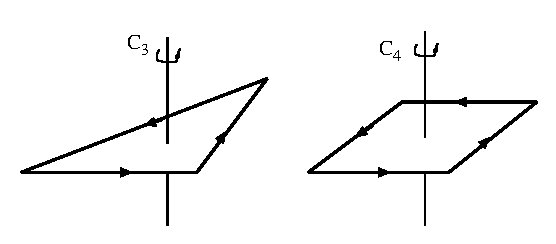
\includegraphics[scale=1.0]{pics/Cn}}

Elementi grupe C$_n$ su rotacije za kuteve 2$\pi r/n$, ($r=0,1,\ldots, n-1$)
oko osi koja okomito probada središte poligona. Usmjerenost
stranica isključuje rotacije oko osi koje leže u ravnini poligona. 
(Iako je poligon ravninski lik ovdje ga zamišljamo u 3D prostoru.)

Specifično svojstvo cikličkih grupa je da je sve elemente grupe moguće
dobiti uzastopnim komponiranjem ("množenjem") jednog od njih sa samim sobom.
Tako npr. uzastopnim komponiranjem rotacije za kut 2$\pi/3$ sa samom sobom dobivamo ostale
dvije rotacije koje sačinjavaju grupu C$_3$: rotaciju za 4$\pi/3$ i
rotaciju za 0 radijana. 
Ukoliko označimo "generirajuću" rotaciju grupe C$_n$ (onu za kut 2$\pi/n$) simbolom 
$c$ onda je skup elemenata grupe
\begin{equation}
 \{c,c^2, \ldots , c^n=e \} \;,
\label{eq:cn}
\end{equation}
odnosno grupu C$_n$ možemo alternativno definirati kao grupu generiranu
elementom $c$ sa svojstvom $c^n=e$ i pisati kao definicioni izraz
\begin{equation}
 {\rm C}_n = \langle c \: | \: c^n=e \rangle \;.
\label{eq:cngp}
\end{equation}
Ovakvo navođenje generatora i njegovih (ili njihovih ako ih ima više, vidi kasnije)
svojstava je kompaktni način definiranja grupe poznat i kao \emph{prezentacija}
grupe. (Što nikako ne treba miješati s \emph{reprezentacijom} grupe što je nevezani
pojam kojeg ćemo kasnije definirati!)

Treću mogućnost za definiciju ove i drugih grupa pruža nam grupna tablica množenja
(poznata i kao Cayleyjeva tablica).
Naime, obzirom da je apstraktna grupa potpuno određena time da se navede
skup elemenata koji je sačinjavaju te time da se potpuno specificira kako
se ti elementi množe (tj. kakva je binarna operacija u grupi), grupu C$_3$, npr.,
je moguće definirati naprosto kao skup elemenata koji zadovoljavaju slijedeću tablicu
množenja:
\begin{equation}
\begin{array}{c|ccc}
g_1\backslash\ g_2 & e & c & c^2 \\ \hline
   e    & e & c & c^2 \\
   c    & c & c^2 & e \\
   c^2    & c^2 & e & c
\end{array}
\label{eq:cntab}
\end{equation}
Konvencija je da prvi redak i stupac tablice odgovaraju množenju
s jediničnim elementom što zapravo čini naslovni redak i stupac
suvišnim i ovu je tablicu moguće i jednostavnije zapisati samo kao
\begin{equation}
\begin{array}{|ccc}
 \hline
 e & c & c^2 \\
 c & c^2 & e \\
 c^2 & e & c
\end{array}
\label{eq:cntabsimple}
\end{equation}

Grupne tablice množenja zadovoljavaju tzv. svojstvo latinskog
kvadrata poznato i kao
\begin{teorem}[Teorem o razmještaju]
Svaki element grupe se pojavljuje jednom i samo jednom u svakom stupcu
ili retku grupne tablice množenja.
\end{teorem}

\emph{Dokaz}: Pretpostavimo suprotno tj. da se u nekom retku
dvaput pojavi isti element, recimo $a$. To znači da je $a$ moguće
dobiti množenjem prvog elementa iz tog retka, neka je to $k$, s
dvama različitim elementima, recimo $m$ i $n$: $km=a$ i $kn=a$. To bi značilo
da je $km=kn$, a egzistencija inverza omogućuje "skraćivanje"
ovakvih relacija tj. množenje slijeva s $k^{-1}$ pa
dobivamo $m=n$ što je kontradiktorno jer smo pretpostavili da su
$m$ i $n$ različiti elementi. Do slične bi kontradikcije dovela
pretpostavka  ponavljanja istog elementa dvaput u istom stupcu.\qed

Treba uočiti da nam binarna operacija definirana tablicom množenja
koja je u standardnom obliku gdje prvi redak i stupac odgovaraju
jediničnom elementu i koja poštuje teorem o razmještaju automatski 
garantira zadovoljavanje tri aksioma grupe: 
\emph{zatvorenost} (u tablici se pojavljuju samo elementi grupe), 
\emph{egzistencija identiteta} (po konstrukciji prvog retka i stupca) i
\emph{egzistencija inverza} (u svakom retku se nužno pojavljuje i 
jedinični element i odgovarajući stupac je onda stupac inverza).
Međutim, svojstvo \emph{asocijativnosti} nije nužno zadovoljeno
i treba ga provjeriti nekim drugim načinom\footnote{Eksplicitna provjera
može biti mukotrpna. Od pomoći je procedura poznata kao Lightov
test asocijativnosti.}.


Ove dvije alternativne definicije grupe putem prezentacije (\ref{eq:cngp}) ili
putem tablice množenja (\ref{eq:cntabsimple}) 
naglašavaju apstraktnu prirodu grupe jer se nigdje ne oslanjaju
na ideju da je C$_3$ grupa simetrija trokuta.

Inače, C$_n$, za $n=2,3,4$ i $6$, spada u kristalografske \emph{točkaste grupe} kakvih
ima ukupno 32\footnote{U trodimenzionalnom prostoru. U dvodimenzionalnom prostoru postoji 10, a u
jednodimenzionalnom prostoru samo dvije točkaste grupe.}. 
Točkaste grupe su grupe prostornih simetrija savršenih beskonačnih
periodičnih kristala koje ostavljaju barem jednu točku nepomičnom. (Za
razliku od npr. translacije za konstantu rešetke koja je isto simetrija
kristala, ali nijednu točku ne ostavlja na mjestu.)
  
Može se pokazati da jedini elementi tih grupa mogu biti kompozicije
rotacija za 60$^\circ$ i 90$^\circ$ te inverzije $\vec{r}\to -\vec{r}$
(cf. \emph{Crystallographic restriction theorem}).
   

\begin{primjer}[Dihedralna grupa D$_n$]
Dihedralna grupa D$_n$ je grupa simetrija rotacija pravilnog poligona s $n$ stranica.
Prema slici

\centerline{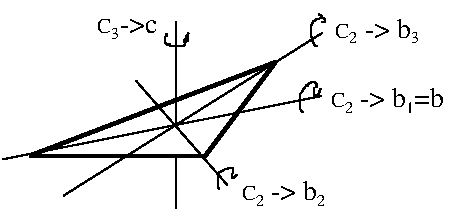
\includegraphics[scale=1.0]{pics/D3}}

vidimo da su elementi grupe rotacije $e, c$ i  $c^2$ baš kao kod grupe C$_n$, te
dodatno rotacije $b_1, b_2$ i $b_3$ za kut 180$^\circ$ oko triju horizontalnih
osi.
\end{primjer}

Uočimo sada neka svojstva množenja u toj grupi. Kao prvo, vrijedi
da je $b_2 = c b_1 c^{-1}$ i kažemo da su $b_2$ i $b_1$ međusobno
\emph{konjugirani} preko elementa $c$. Da je to tako vidi
se iz slike:

\centerline{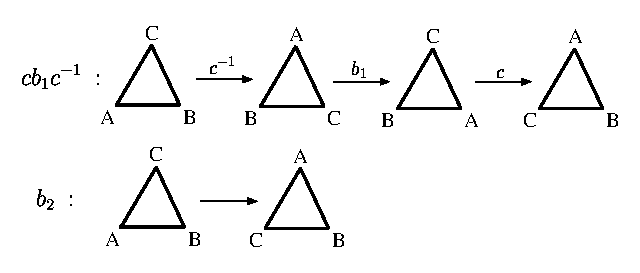
\includegraphics[scale=1.0]{pics/cbc}}

Na sličan način se možemo uvjeriti da je $b_2 = b_1 c $
i $b_3 = b_1 c^2 $, odnosno da 
$c$ i $b\equiv b_1$ generiraju sve ostale transformacije pa
elemente grupe možemo zapisati kao
\begin{equation}
 \{e,c,c^2,b,bc,bc^2\} \;.
\label{eq:d3el}
\end{equation}
To sugerira da bismo grupu D$_3$ mogli probati definirati prezentacijom
\begin{equation}
    {\rm D}_3 \stackrel{?}{=} \langle c, b \: | \: c^3 = b^2 = e \rangle \;,
\label{eq:d3gp1}
\end{equation}
no ova definicija nije kompletna jer nam nedostaje još
i pravilo za komutiranje elemenata (koje nam nije trebalo
za grupu C$_n$ koja je Abelova). Njega dobijemo tako da
iskombiniramo dvije gore dobivene relacije: 
$b_2 = c b_1 c^{-1} = b c$ i pomnožimo zdesna s $c$:
\begin{equation}
c b = b c^2  \;.
\label{eq:d3com}
\end{equation}
Ova relacija sad omogućuje da proizvoljan umnožak elemenata
grupe (npr. $b c b^2 c^5 b$ svedemo na oblik $b^\alpha c^\beta$ gdje
je $\alpha<2$ i $\beta<3$, tj. na jedan od elemenata iz (\ref{eq:d3el}).
Za kompaktan zapis prezentacije grupe D$_3$ koji će se onda moći
lako generalizirati i na ostale D$_n$ grupe, množimo gornju
komutacijsku relaciju (\ref{eq:d3com}) slijeva s $b$ i zdesna s $c$
i dobivamo  $ bcbc \equiv (bc)^2 = b^2 c^3 = e$ pa možemo
pisati
\begin{equation}
 {\rm D}_3= \langle c,b \: | \: c^3 = b^2 = (bc)^2 = e \rangle \;.
\label{eq:d3gp}
\end{equation}
Ova definicija se generalizira ovako (vidi zadatke)
\begin{equation}
 {\rm D}_n= \langle c,b \: | \: c^n = b^2 = (bc)^2 = e \rangle \;,
\label{eq:dngp}
\end{equation}
ili, ekvivalentno i praktičnije za komutiranje elemenata prilikom množenja
\begin{equation}
    {\rm D}_n= \langle c,b \: | \: c^n = b^2 = e, cb = b c^{n-1} \rangle \;,
\label{eq:dngpcom}
\end{equation}
što onda sadrži i definiciju grupe
D$_2$ poznate i kao
\emph{Kleinova četvorna grupa} (njem. \emph{Vierergruppe}), 
za koju nemamo odgovarajući poligon kao objekt grupe simetrija.


\section{Podgrupe}

Za operacije s grupama i njihovu klasifikaciju centralni je pojam \emph{podgrupe}:

\begin{definicija}[Podgrupa]
Podgrupa $H$ grupe $G$ je neprazni podskup $H\subset G$ koji i sam
tvori grupu obzirom na grupnu operaciju definiranu na $G$.
\end{definicija}

Svaka grupa ima trivijalne podgrupe $H=\{e\}$ i $H=G$, a
podgrupu koja je različita od ovih dviju trivijalnih
zovemo \emph{prava} podgrupa.

\begin{primjer} \label{th:c2c3}
C$_2$=\{e, b\} i C$_3$=\{e, c, c$^2$\} su prave podgrupe od D$_3$
\end{primjer}

\begin{primjer}
Grupa translacija i točkasta grupa su podgrupe grupe svih prostornih
simetrija kristala.
\end{primjer}

\begin{definicija}[Susjedna klasa]
Lijeva susjedna klasa (engl. coset) podgrupe $H$ obzirom na element
$g\in G$ je skup
\begin{displaymath}
     gH=\{gh \td h\in H\}
\end{displaymath}
\end{definicija}

Odnos pripadnosti elementa $g_1$ lijevoj susjednoj klasi obzirom na element $g_2$,  
$g_1 \in g_2 H$, uspostavlja \emph{relaciju ekvivalencije}%
\footnote{Općenito, \emph{relacija ekvivalencije} je binarna relacija $a\sim b$ između
elemenata nekog
skupa koja ima slijedeća svojstva
\begin{enumerate}
\item $a\sim a \quad \forall a$ \qquad (refleksivnost)
\item $a\sim b \imp b\sim a$   \qquad (simetričnost)
\item $a\sim b \quad \textrm{i}\quad  b\sim c \imp a\sim c$  \qquad (tranzitivnost)
\end{enumerate}
Primjeri relacija ekvivalencije su: "osoba $a$ je rođena na isti dan kad i osoba $b$"
ili "trokut $a$ je sličan trokutu $b$", dok npr. "broj $a$ je veći ili jednak
broju $b$" nije relacija ekvivalencije jer nije simetrična.
(Ona je antisimetrična. Binarna relacija na skupu koja je refleksivna, antisimetrična
i tranzitivna zove se \emph{relacija uređaja}.)
Svaka relacija ekvivalencije cijepa skup na disjunktne podskupove 
koji se zovu \emph{klase ekvivalencije}.} između ta dva elementa u grupi G, $g_1 \sim g_2$.
To između ostalog znači i da bilo koji element klase možemo jednako koristiti
kao reprezentanta klase tj. da ako je $g_k \in gH$ onda je $g_{k}H = gH$.

Susjedne klase po nekoj podgrupi $H$ su međusobno disjunktne i
zahvaljujući Teoremu o razmještaju sve imaju isti broj elemenata (jednak redu od $H$)
pa tako definiraju jednu particiju grupe G:

\centerline{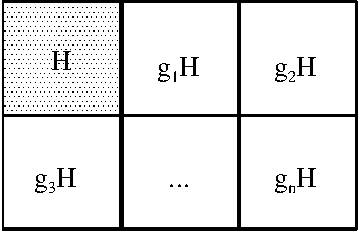
\includegraphics[scale=1.0]{pics/lagrange}}

Na slici je kao prva postavljena lijeva susjedna klasa po jediničnom
elementu $eH = H$. Zbog navedene disjunktnosti klasa i jedinstvenosti
jediničnog elementa ostale susjedne klase naravno ne sadrže jedinični element i
samim time one nisu podgrupe. 
Promatrajući ovu sliku lako se uvjerimo u točnost Lagrangeovog
teorema:

\begin{teorem}[Lagrange]
Red podgrupe dijeli red grupe.
\end{teorem}

Tako u Primjeru \ref{th:c2c3} redovi podgrupa C$_2$ i C$_3$, 2 i 3, dijele red
grupe D$_3$, 6. Skup čiji su elementi predstavljeni kvadratičima na gornjoj slici
ima svoj naziv:

\begin{definicija}[Kvocijentni skup]
Skup svih različitih lijevih susjednih klasa 
\begin{displaymath}
      G/H \equiv \{gH \td g\in G\}
\end{displaymath}
zove se \emph{lijevi kvocijentni skup grupe} $G$ po podgrupi $H$.
\end{definicija}

Potpuno analogno se definiraju \emph{desna susjedna klasa} $Hg$
i \emph{desni kvocijentni skup} $H\backslash G$.

\begin{primjer}[D$_3$]
    Promotrimo podgrupu $H=\mathrm{C}_3=\{e, c, c^2\}$ grupe $G=\mathrm{D}_3$.
Dvije lijeve susjedne klase su
\begin{enumerate}
\item $eH=H=\{e, c, c^2\}$ \; \text{i}
\item $bH=\{b, bc, bc^2\}$ \;,
\end{enumerate}
a kvocijentni skup je $\mathrm{D}_3/\mathrm{C}_3=\{eH, bH\}$. Postoji i kvocijentni 
skup $\mathrm{D}_3/\mathrm{C}_2$
\end{primjer}

\begin{definicija}[Normalna podgrupa]
Podgrupa za koju vrijedi $gH=Hg$, $\forall g\in G$, zovemo
\emph{normalna} ili \emph{invarijantna}.
\label{tm:normalnapodgrupa}
\end{definicija}

\begin{primjer}[$\mathrm{D}_3$]
    $G=\mathrm{D}_3$, $H=\mathrm{C}_3$. Eksplicitnim množenjem se uvjerimo da
    je $b\mathrm{C}_3 = \mathrm{C}_3 b$, a za ostale elemente $g\in \mathrm{D}_3$ jednakost
    lijevih i desnih susjednih klasa je trivijalna.
    Dakle, $\mathrm{C}_3$  je normalna podgrupa od $\mathrm{D}_3$. S druge strane
    $\mathrm{C}_2 = \{e, b\}$ nije normalna podgrupa od $\mathrm{D}_3$
    jer npr. $c \mathrm{C}_2 \neq \mathrm{C}_2 c$.
\end{primjer}

Očito je da su za normalnu podgrupu $H$ lijevi i desni kvocijentni skupovi
identični  $G/H$ = $H\backslash$G.

Zanimljivo je pitanje u kojim okolnostima i sam kvocijentni skup čini grupu.
Za to je potrebno definirati binarnu operaciju elemenata kvocijentnog
skupa tj. "množenja" susjednih klasa.
Prirodno je pokušati s definicijom množenja dvije klase $A$ i 
$B$ "svaki element sa svakim":
\begin{equation}\label{eq:ABmult}
    A B =\{ab \td a \in A \:\text{i}\: b \in B\} \;.
\end{equation}
Pitanje je međutim predstavlja li ovako definirano množenje skupova $A$ i $B$
konzistentnu definiciju množenja susjednih klasa tj. je li $AB$ nužno susjedna
klasa, ukoliko su to $A$ i $B$? To zahtijeva prvi aksiom definicije
grupe. Lako se možemo uvjeriti da tako definirano množenje \emph{ne} funkcionira
na kvocijentnom skupu $\mathrm{D}_3 / \mathrm{C}_2$, gdje je $\mathrm{C}_2 = \{e, b\}$.
Npr. umnožak susjednih klasa $e\mathrm{C}_2 = \{e, b\}$ i $c\mathrm{C}_2=\{c, bc^2\}$
je $\{e, bc, bc^2, b^2 c^2 = c^2\}$ što je skup koji nije susjedna klasa!
S druge pak strane množenje susjednih klasa u kvocijentnom skupu
$\mathrm{D}_3 / \mathrm{C}_3$ uvijek rezultira susjednom klasom. Razlog tome je
što je $\mathrm{C}_3$ \emph{normalna} podgrupa, a za normalnu podgrupu $H$ 
množenje klasa možemo provesti kao:
\begin{equation}
       (g_1H)(g_2H) = g_1 (H g_2) H = g_1 (g_2 H) H = g_1 g_2 H H
       = (g_1 g_2) H\;,
\end{equation}
gdje smo u drugom koraku iskoristili normalnost podgrupe $H$ i gdje je
$(g_1 g_2) H$ nužno susjedna klasa jer je $g_1 g_2 \in G$.
Lako se uvjeriti da su i ostali aksiomi grupe zadovoljeni pa zaključujemo
da kvocijentni skup po normalnoj podgrupi čini grupu koju zovemo
\emph{kvocijentna grupa}\footnote{Nešto je teže
    uvjeriti se u činjenicu da bi i drugačiji pokušaji definiranja množenja
    susjednih klasa od (\ref{eq:ABmult}) doveli do nužnosti da podgrupa
bude normalna. Npr. mogli bi umjesto oslanjanja na (\ref{eq:ABmult}) 
\emph{definirati} množenje susjednih klasa kao $(g_1 H) \ast (g_2 H) = (g_1 g_2) H$.
Tako bi prvi aksiom grupe naizgled bio osiguran samom definicijom binarne operacije.
No pokazuje se da je ovakva definicija množenja susjednih klasa konzistentna, u smislu
da ne ovisi o izboru reprezentirajućih elemenata $g_1$ i $g_2$, i opet samo ako je
podgrupa normalna.}


\begin{primjer}[$\mathrm{D}_{3}$/$\mathrm{C}_3$]
Tablica množenja u ovom kvocijentnom skupu je dana relacijama
\begin{align}
    (e\mathrm{C}_3)(e\mathrm{C}_3) &= ee \mathrm{C}_3 = e\mathrm{C}_3\\
    (e\mathrm{C}_3)(b\mathrm{C}_3) &= b\mathrm{C}_3  \\
    (b\mathrm{C}_3)(e\mathrm{C}_3) &= b\mathrm{C}_3  \\
    (b\mathrm{C}_3)(b\mathrm{C}_3) &= e\mathrm{C}_3 
\end{align}

Lijevi i desni kvocijentni skupovi su jednaki
\begin{align*}
{\rm D}_{3}/{\rm C}_3 &= \{\{e,c,c^2\}, \{b, bc, bc^2\}\} \\
{\rm C}_3\backslash{\rm D}_{3} &= \{\{e,c,c^2\}, \{b, cb=bc^2, c^2b=bc\}\}
    = D_{3}/C_3
\end{align*}
i imaju grupnu strukturu jednaku grupi $\mathrm{C}_2$.
\label{pr:D3oC3}
\end{primjer}

S druge strane $\mathrm{C}_2$ nije normalna, lijevi i desni kvocijentni
skupovi
\begin{align*}
{\rm D}_{3}/{\rm C}_2 &= \{\{e,b\}, \{c, cb=bc^2\}, \{c^2, c^2b=bc\}\} \\
{\rm C}_2\backslash{\rm D}_{3} &= \{\{e,b\}, \{c, bc\}, \{c^2, bc^2\}\}
    \neq {\rm D}_{3}/{\rm C}_2
\end{align*}
nisu jednaki i $\mathrm{D}_{3}$/$\mathrm{C}_2$ nije grupa.

Grupe koje nemaju normalnih podgrupa zovu se \emph{jednostavne},
a one koje nemaju normalnih Abelovih podgrupa zovu se \emph{polujednostavne}.

Za normalne grupe iz definicije \ref{tm:normalnapodgrupa} slijedi odmah i
da je $g H g^{-1} = H, \forall g\in G$. Zanimljivo je promatrati djelovanje
ove operacije $g \ldots g^{-1}$ i na skupove koji nisu podgrupa te
na pojedine elemente grupe:

\begin{definicija}[Konjugirani elementi]
Dva elementa $a$ i $b$ grupe $G$ su \emph{konjugirani} ukoliko
postoji $g\in G$ takav da je $a=gbg^{-1}$.
\label{tm:konjugacija}
\end{definicija}

Konjugacija je također relacija ekvivalencije:
\begin{enumerate}
\item $a=e^{-1} a e  \imp a\sim a$
\item $a=g^{-1} b g  \imp  b= g^{-1} a (g^{-1})^{-1}$
\item $a=g b g^{-1}$, $b=hch^{-1}$, \\
         $a=ghch^{-1}g^{-1}=(gh)c(gh)^{-1}$, $gh\in G$
  
\end{enumerate}


Konjugacija (baš kao i svaka relacija ekvivalencije) definira
particiju skupa na klase.
\begin{displaymath}
   \text{klasa od $a$} = \{ b \td b=gag^{-1},\quad g\in G\}
\end{displaymath}

Klasa od $e=\{e\}$ što znači da klase, izuzev ove trivijalne, nisu podgrupe.

Za Abelove grupe svaki element je klasa za sebe.

Kako normalne podgrupe zadovoljavaju $gHg^{-1}=H$, $\forall g\in G$, slijedi
da su one sastavljenje od \emph{cijelih} klasa konjugacije.

\begin{primjer}[D$_3$]
Tri klase konjugacije  od D$_3$ su:
\begin{enumerate}
\item $(e)$
\item $(c, c^{2})$
\item $(b, bc, bc^2)$
\end{enumerate}
i odgovaraju rotacijama za različite kuteve: $0^\circ$, $120^\circ$ i
$180^\circ$. Konjugirajući elementi
preslikavaju međusobno osi rotacije. Normalna podgrupa $C_3$ se
sastoji od cijelih klasa (prve dvije), dok podgrupa $C_2=\{e,b\}$ nema
to svojstvo i nije normalna.
\end{primjer}


\section{Homomorfizam i izomorfizam grupa}

Vidjeli smo u primjeru \ref{pr:D3oC3} kako kvocijentna grupa $\mathrm{D}_3/\mathrm{C}_3$
ima isti broj elemenata i istu tablicu množenja kao grupa $\mathrm{C}_2$. Dakle u
apstraktnom smislu teorije grupa te su grupe identične.  Za prepoznavanje takvih
situacija, umjesto uspoređivanja grupnih tablica množenja pogodnije je identificirati
preslikavanje s jedne grupe na drugu koje "čuva" grupnu strukturu. Takvo preslikavanje
se naziva \emph{homomorfizam}:
\begin{definicija}[Homomorfizam]
Neka su $G$ i $H$ grupe, a $f:G\to H$ preslikavanje koje komutira
s grupnom operacijom tj. za koje vrijedi
\begin{displaymath}
      f(ab)=f(a)f(b) \quad \forall a,b\in G \;.
\end{displaymath}
Onda kažemo da je $f$ \emph{homomorfizam} grupe $G$ u grupu $H$.
\end{definicija}

\begin{primjer}
    Preslikavanje s grupe $\mathrm{D}_3$ na kvocijentnu grupu
    $\mathrm{D}_3/\mathrm{C}_3$ definirano kao 
    \[
        f(g) = g\mathrm{C}_3 \,,
    \] je homomorfizam jer
    \[
        f(a) f(b) = (a \mathrm{C}_3) (b \mathrm{C}_3 ) =
        (a b) \mathrm{C}_3 = f(a b)
    .\] 
\end{primjer}
\begin{primjer}
    Preslikavanje s grupe $\mathrm{C}_3$ na trivijalnu grupu $\mathrm{C}_1 = \{e\}$
    koja sadrži samo jedinični element, definirano kao $f(g) = e,
    \forall g\in\mathrm{C}_3$, je homomorfizam.
    Vidimo da homomorfizam općenito ne mora biti injekcija tj. da se više
    elemenata može preslikavati u isti element.
    \label{pr:C3toC1}
\end{primjer}

Homomorfizam koji je i bijekcija zovemo \emph{izomorfizam} i
pišemo $A\cong B$ ili $A=B$.

Izomorfne grupe su s apstraktnog stanovišta jednake (imaju
istu tablicu množenja).

\begin{primjer}[C$_2$]
Grupa C$_2$ je, osim već spomenutog izomorfizma s
kvocijentnom grupom $\mathrm{D}_3/\mathrm{C}_3$, izomorfna i
s grupama $(\{1, -1\},\cdot$) i
$\left(\left\{
\begin{pmatrix}
1 & 0 \\ 0 & 1
\end{pmatrix},
\begin{pmatrix}
0 & 1 \\ 1 & 0
\end{pmatrix}
\right\},\cdot\right)$.
\end{primjer}

\emph{Slika} homomorfizma $f(A)$ (skup svih elemenata u $B$ koji imaju original u $A$) 
je podgrupa od $B$. Uvjerite se u to.


\begin{figure}[htpb]
    \centering
    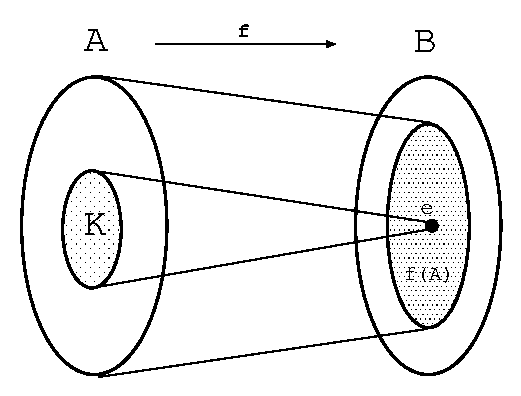
\includegraphics[width=0.6\textwidth]{pics/homomorfizam}
    \caption{Kernel $K$ homomorfizma $f:A\toB$ je podgrupa grupe $A$,
    a slika $f(A)$ homomorfizma je podgrupa grupe $B$.}
    \label{fig:kernelslika}
\end{figure}


Slika $f(e_A)$ jediničnog elementa $e_A$ iz $A$ je jedinični element $e_B$ u $B$ jer
množenjem relacije
$$ f(e_A) f(b) = f(e_A b) = f(b) $$
s desna s $f(b)^{-1}$ dobivamo
$$ f(e_A) = f(b) f(b)^{-1} = e_B \;. $$
No moguće je da se i drugi elementi iz $A$ osim jediničnog $e_A$ preslikavaju u 
jedinični element $e_B$ u $B$ (u primjeru \ref{pr:C3toC1} se svi tako preslikavaju).
\emph{Kernel} homomorfizma se naziva skup svih elemenata od $A$ koji se
preslikavaju u jedinični element iz $B$.
$$ K \equiv {\rm ker}(f) \equiv \{ k\in A \; | \; f(k) = e_B \} \;. $$
Kernel od $f:A\to B$ je normalna podgrupa od $A$. Uvjerite se u to.

Kernel je iznimno korisna podgrupa, između ostalog i zahvaljujući sljedećem
važnom teoremu:
\begin{teorem}[Teorem o izomorfizmu]
\label{th:izomorfizam}
Ako je $f:G\to G'$ homomorfizam s kernelom $K$, onda vrijedi
\begin{enumerate}
\item Svaki element susjedne klase $gK$ se preslikava u isti element $f(g)$.
\item Slika homomorfizma $f(G)$ je izomorfna kvocijentnoj grupi po kernelu $G/K$.
\end{enumerate}
\end{teorem}
(Skup $G/K$ je grupa jer je $K$ normalna podgrupa.)

\emph{Dokaz}$^{*}$\secret{Cornwell '84, 2.6}: Pridruživanje je $f(g)\leftrightarrow gK$.
Pokažimo da je to pridruživanje dobro definirano i bijekcija te da čuva grupnu
strukturu.

- $f(g)\mapsto gK$ je dobro definirano jer je gK jedinstven: $f(g)=f(g')$
  $\imp f(g'g^{-1})=f(g')f(g^{-1})=f(g)f(g)^{-1}=e
   \imp g'g^{-1}\equiv k\in K, g'=kg \imp gK=g'K$
(Zadnja implikacija slijedi iz toga da $\forall k_1 \in K, gk_1 = 
g' k^{-1}k_1 \in g' K$)

\vspace*{1ex}

\centerline{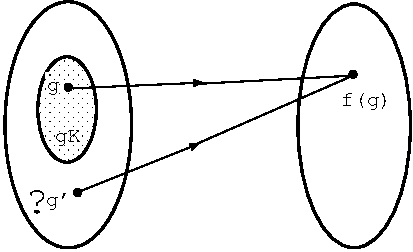
\includegraphics[scale=0.8]{pics/homo1}}

- $gK\mapsto f(g)$ je dobro definirano jer ne ovisi o izboru
  elementa $g$ iz $K$: $g,g'\in gK \imp g'g^{-1}\in K \imp
   \imp f(g'g^{-1})=e \imp f(g')f(g^{-1})=e \imp f(g')=f(g)$

\vspace*{1ex}

\centerline{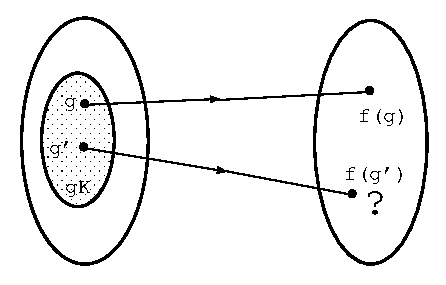
\includegraphics[scale=0.8]{pics/homo2}}

- injekcija u oba smjera $\imp$ bijekcija

- Čuvanje grupne strukture: f(g)f(g') se preslikava u (gK)(g'K) jer \\
  f(g)f(g')=f(gg')=gg'K=(gK)(g'K)
  
\vspace*{1ex}

\centerline{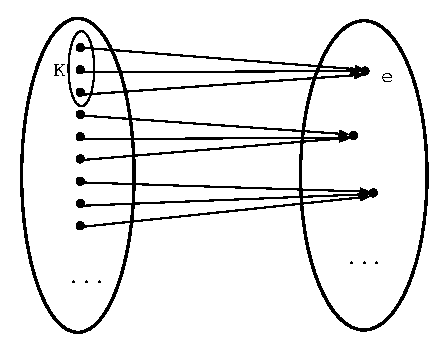
\includegraphics[scale=1.0]{pics/homo3}}

\secret{Primjer: $D_3$: $C_3\to e$, a ostali u $c$ iz $C_2$
 $\imp f(D_3) = C_2 = D_3/C_3$}

Jedan korolar ovog teorema je da je svaki element $g'$ iz $G'$ slika
istog broja elemenata iz G (zato jer susjedne klase moraju imati
isti broj elemenata). Drugi korolar je da je $f$ izomorfizam ako i
samo ako je kernel $K=\{e\}$.


\subsection*{Zadaci}

\begin{enumerate}[label=\arabic{chapter}.\arabic*.]
\item Dokažite da su jedinični i inverzni element grupe jedinstveni.
\item Konstrukcijom grupne tablice množenja pokažite da postoji samo
jedna grupa reda 3.
\item Na isti način kao u prošlom zadatku pokažite da postoje samo
dvije grupe reda 4.
\item Grupa je Abelova ako i samo ako je njena grupna tablica množenja simetrična.
Dokažite da i za grupe koje nisu Abelove razmještaj jediničnih elemenata u tablici
mora biti simetričan.
\item Dokažite da je grupa u kojoj je svaki element samom sebi inverz nužno Abelova.
\item Uvjerite se da je grupa simetrija pravilnog poligona s $n$ neusmjerenih
stranica izomorfna grupi D$_n$=gp($c,b$) $\quad c^n = b^2 = (bc)^2 = e $.
(Naputak: Odredite transformacije poligona koje odgovaraju elementima $c$ i
 $b$, pa se uvjerite da one zadovoljavaju $c^n = b^2 = (bc)^2 = e $. Usporedite
broj elementa grupa.)\label{Dn}
\item Centar $Z$ grupe $G$ je skup svih elemenata koji komutiraju sa svakim
elementom grupe tj. $Z=\{z\in G \td zg=gz \forall g\in G\}$. Pokažite da
je $Z$ normalna Abelova podgrupa od $G$.
\item Odredite klase konjugacije grupe D$_4$.
\item Pokažite da su sve grupe s prostim brojem elemenata ciklične.
\item \emph{Red} elementa $a$ grupe $G$ je najmanji $n$ takav da je $a^n=e$.
Pokažite da je red svih elemenata jedne klase konjugacije isti.
\item Postoji li netrivijalni homomorfizam s grupe D$_4$ na grupu D$_3$?
\item Pokažite da je kvocijentna grupa $\mathbb{Z}/\mathbb{Z}_e$
izomorfna grupi C$_2$, gdje je $\mathbb{Z}_e$ grupa parnih cijelih brojeva.
\item Promotrite grupu nesingularnih kvadratnih $n\times n$ 
matrica $G=\{M\}$. Pokažite da je $f(M)=\det M$ homomorfizam.
\end{enumerate}
